\documentclass{magnoliaold}

\magtex{tex_driver={pdftex},
        tex_packages={xypic}}
\magfiche{document_nom={Fonction},
          auteur_nom={François Fayard},
          auteur_mail={francois.fayard@auxlazaristeslasalle.fr}}
\magcours{cours_matiere={python},
          cours_niveau={mpsi},
          cours_chapitre_numero={3},
          cours_chapitre={Fonction}}
          \magmisenpage{misenpage_presentation={tikzvelvia},
          misenpage_format={a4},
          misenpage_nbcolonnes={1},
          misenpage_preuve={non},
          misenpage_sol={non}}

\maglieudiff{}
\magprocess

\usepackage{minted}
\usemintedstyle{xcode}

\begin{document}
%BEGIN_BOOK
\hfill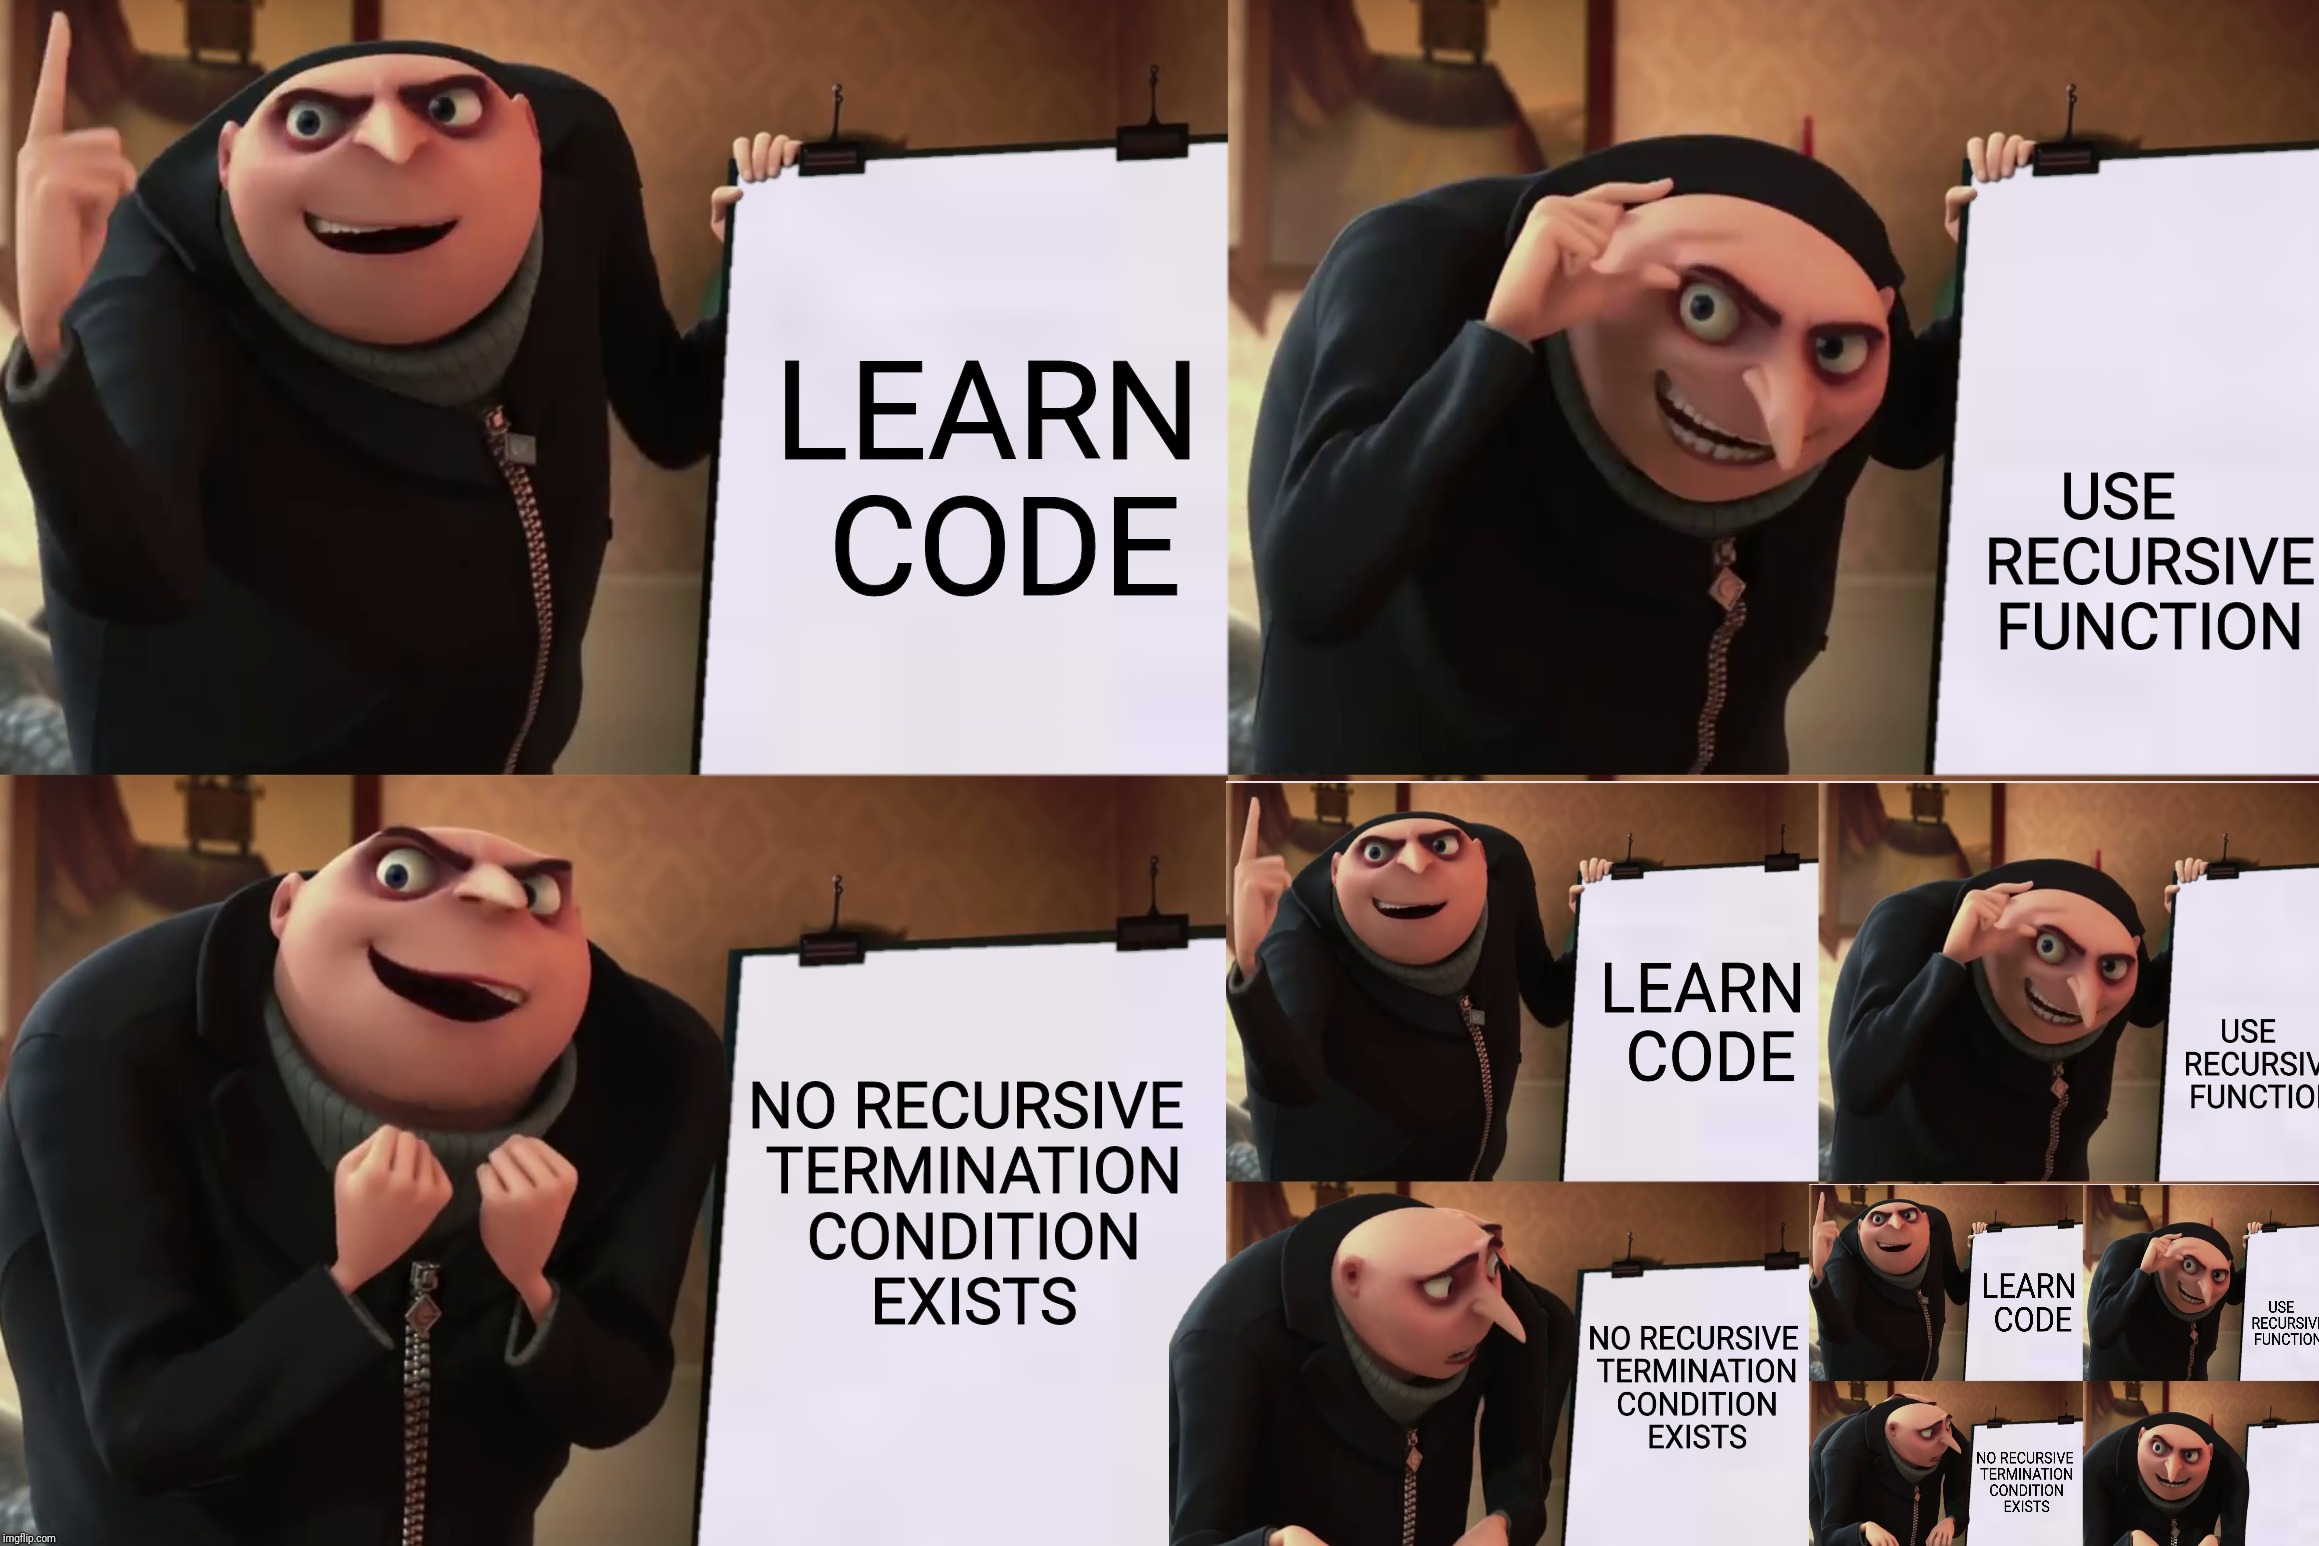
\includegraphics[width=0.5\textwidth]{../../Commun/Images/python-cours-recursion}
\magtoc

\section{Fonction}

\subsection{Fonction}

La syntaxe générale d'une fonction en Python est
% \begin{francois}
\begin{pythoncode}
def (*@\textcolor{purple}{nom\_fonction}@*)((*@\textcolor{purple}{arg1, ..., argn}@*)):
    (*@\textcolor{purple}{bloc....................}@*)
    (*@\textcolor{purple}{..........d'instructions}@*)
\end{pythoncode}

\noindent
Le bloc d'instruction a pour vocation soit~:
\begin{itemize}
\item de calculer une nouvelle valeur qui est renvoyée à l'aide
de l'instruction \verb_return_.
\item d'avoir un effet de bord comme afficher du texte
sur la sortie standard.
\end{itemize}
Les arguments \verb_arg1_, $\ldots,$ \verb_argn_ sont appelés
\emph{arguments formels}. On appelle une fonction à l'aide de la syntaxe
\verb!nom_fonction(arg1, ..., argn)!; les valeurs des expressions
\verb_arg1_, $\ldots,$ \verb_argn_ sont appelées \emph{arguments effectifs}.\\

Une fonction
renvoie toujours \emph{une unique} valeur. On utilise pour cela l'instruction \verb!return!. Lorsqu'on souhaite seulement effectuer un effet de bord, on renvoie \verb!None!, ce que
Python fait automatiquement s'il ne rencontre pas de \verb!return!.\\

Python étant un langage de programmation à \emph{typage dynamique}, nous n'avons pas besoin de
préciser, ni les types des arguments, ni le type de la valeur de retour. Cette caractéristique
du langage nous permet d'avoir des fonctions acceptant des arguments effectifs de types différents~:

\begin{pythoncodeline}
def f(x):
    return x + 1
\end{pythoncodeline}

\begin{pythoncode}
In [1]: f(2)
Out[1]: 3

In [2]: f(2.0)
Out[2]: 3.0
\end{pythoncode}

\noindent
L'idée est que $f$ peut accepter comme argument n'importe quel type que l'on peut
ajouter à 1. En Python, les types \verb_int_ et \verb_float_ sont de bons
candidats. On peut dire que la fonction $f$ accepte un nombre et renvoie un nombre.
On dit que Python fonctionne avec le principe du \og duck typing \fg dont la devise est~:
\og If it walks like a duck and it quacks like a duck, then it must be a duck \fg. Autrement
dit, dans notre cas, si $f(x)$ a un sens, c'est que $x$ est un nombre.\\

Cependant, le plus souvent, nous définirons des fonctions qui ont vocation
à être utilisées avec des paramètres d'un type donné. Dans ce cas, la valeur
de retour est généralement aussi d'un type déterminé. Par exemple, la fonction

\begin{pythoncodeline}
def est_pair(n):
    return n % 2 == 0
\end{pythoncodeline}

\noindent
est pensée pour prendre en entrée un entier; elle renvoie alors un booléen. On dit que la signature
de cette fonction est \verb!est_pair(n: int) -> bool!. En Python, si le bloc
d'instructions commence par une chaine de caractères, elle est utilisée comme
documentation. L'utilisation des triples \verb_"_ permet 
de rentrer des chaines de caractères qui  s'étirent sur plusieurs lignes.
Il est coutume d'utiliser de telles chaines pour la documentation; on les appelle
\emph{docstrings}.

\begin{pythoncodeline}
def est_pair(n):
    """est_pair(n: int) -> bool"""
    ans = (n % 2 == 0)
    return ans
\end{pythoncodeline}

\noindent
Cette signature est présente uniquement à titre de documentation et
n'est pas lue par Python. Par exemple, rien n'empêche la fonction
\begin{pythoncodeline}
def suivant(n):
    """suivant(n: int) -> int"""
    return n + 1
\end{pythoncodeline}
d'être appelée avec un nombre flottant. Cependant, les fonctions que nous écrirons ne s'utiliseront
qu'avec les types suggérés par la docstring.\\

Une fonction ne peut renvoyer qu'une seule valeur, ce qui est parfois problématique.
Supposons par exemple que l'on souhaite écrire une fonction qui nous donne l'heure en 
fonction du nombre de secondes qui se sont écoulées depuis minuit. On doit pour cela renvoyer
trois entiers~: $h$, $m$ et $s$. Pour cela, on choisit de renvoyer un tuple
formé de 3 entiers. Une affectation simultanée permet de déconstruire le tuple lors de
l'appel d'une telle fonction.

\begin{pythoncodeline}
def heure(n):
    """heure(n: int) -> tuple[int, int, int]"""
    s = n % 60
    n = n // 60
    m = n % 60
    h = n // 60
    return h, m, s  
\end{pythoncodeline}

\begin{pythoncode}
In [3]: h, m, s = heure(42000)
\end{pythoncode}

% \begin{exoUnique}
% \exo Écrire une fonction \texttt{est\_pair} qui prend pour argument un entier \verb_n_ et
%   qui renvoie le booléen disant si cet entier est pair ou non.  On proposera deux versions,
% 	l'une utilisant une variable auxiliaire pour stocker le résultat à renvoyer, et l'autre
% 	sans.
% 	\begin{sol}
% 		\begin{pythoncode}
% 		def est_pair(n):
% 				"""Renvoie le booléen disant si nest pair"""
% 				if n % 2 == 0:
% 						rep = True 
% 				else:
% 						rep = False
% 				return(rep)
				
% 		def est_pair(n):
% 				"""Renvoie le booléen disant si n est pair"""\\
% 				return( n % 2 == 0 )
% 		\end{pythoncode}
% 		\end{sol}
% \end{exoUnique}





% \subsection{Arguments multiples}

% Une fonction peut prendre en entrée des arguments multiples. Par exemple, le calcul du
% pgcd de deux entiers positifs peut se faire par la fonction~:

% \begin{pythoncode}
% >>> def pgcd(a, b):
%         while b != 0:
%             c = a % b
%             a = b
%             b = c
%         return a
% >>> pgcd(21, 42)
%  7
% \end{pythoncode}

% Une fonction peut avoir autant d'arguments que l'on le souhaite. Elle peut même n'avoir
% aucun argument.

% \begin{pythoncode}
% >>> def greetings():
%         return "Bonjour"
% \end{pythoncode}




% Afin de bâtir des logiciels complexes, il est essentiel de décomposer notre programme
% en briques logicielles indépendantes. Les fonctions nous permettent une telle décomposition.
% Dans sa forme la plus simple, une fonction prend en entrée une valeur et renvoie une valeur
% calculée à partir de la valeur d'entrée. Par exemple, la fonction

% \begin{pythoncode}
% >>> def carre(n):
%         return n * n
% \end{pythoncode}

% \noindent prend en entrée la valeur \verb_n_ et renvoie la valeur \verb_n * n_. On
% accède ensuite à la fonction de la manière suivante~:

% \begin{pythoncode}
% >>> carre(3)
%  9
% \end{pythoncode}

% \noindent Bien entendu, il est possible d'utiliser le résultat renvoyé par une fonction
% à l'intérieur d'une expression.

% \begin{pythoncode}
% >>> carre(3) + carre(4)
%  25 
% \end{pythoncode}

% \noindent Ces fonctions sont dites pures, dans la mesure où elles ne changent pas l'état
% du système. Attention, ce n'est pas la fonction qui a choisi d'afficher son résultat, mais
% la boucle interactive qui a appelé la fonction \verb_print_ sur le résultat obtenu en
% évaluant l'expression. Les fonctions pures n'ont aucun effet de bord et le résultat qu'elles
% renvoient ne dépend pas de l'état du système. Elles sont donc très proches des fonctions
% mathématiques.\\

% Une fonction peut utiliser des variables dites \emph{locales} pour produire le résultat
% demandé. Par exemple, la fonction

% \begin{pythoncode}
% >>> def est_premier(n):
%         if n <= 1:
%             res = False
%         else:
%             res = True
%             for k in range(2, n):
%                 if n % k == 0:
%                     res = False
%         return res
% >>> est_premier(19)
%  True
% \end{pythoncode}

% \noindent renvoi \verb_True_ si l'entier passé en paramètre est premier et \verb_False_
% dans le cas contraire. L'algorithme teste tous les nombres $2, 3,\ldots, n-1$ et si un de ces
% nombres est un diviseur de $n$, la variable \verb_res_ est changée en \verb_False_. La
% valeur de cette variable est ensuite renvoyée.\\

% L'instruction \verb_return_ interrompt le flot d'instructions de la fonction et renvoie donc
% la valeur indiquée par le premier \verb_return_ rencontré. La fonction précédente peut donc
% se simplifier en~:

% \begin{pythoncode}
% >>> def est_premier(n):
%         if n <= 1:
%             return False
%         for k in range(2, n):
%             if n % k == 0:
%                 return False
%         return True
% \end{pythoncode}

% \noindent Cependant, pour des raisons de lisibilité, il est préférable de ne pas trop
% multiplier les \verb_return_ et donc les points de sortie.

% Fonctions appelant d'autres fonctions

% \begin{exercicepython}{}
% Soit les fonctions définies en Python par~: 
% \begin{pythoncode}
% def f(n):
%     res = 0
%     for i in range(1, n + 1):
%         res = res + 2 * i
%     for j in range(1, n + 1):
%         res = res + 3 * j
%     return(res)
% \end{pythoncode}

% \begin{pythoncode}
% def g(n):
%     res = 0
%     for i in range(1, n + 1):
%         for j in range(1, n + 1):
%             res = res + 2 * i + 3 * j
%     return(res)
% \end{pythoncode}

% \begin{questions}
% \question Que font ces fonctions~? 
% \question Exprimer en fonction de $n$, le nombre d'additions effectuées par chacune de ces deux fonctions.
% \end{questions}
% \end{exercicepython}

% \begin{exercicepython}{}
% On cherche à créer une fonction \verb_binome_ qui pour $n$ et $p$ entiers renvoie~:

%  \[\begin{pmatrix} n \\p \end{pmatrix}= \begin{cases}
%  \dfrac{n!}{p! (n-p)!} & \text{si $0 \leq p \leq n$}\\
%  0  & \text{sinon}
%  \end{cases}.\]

%  \begin{questions}
% \question   On note $H_{i}$ l'hypothèse  \og \verb_res_ contient $(i-1)!$ \fg. Compléter les fonctions suivantes de sorte que la fonction \verb+binome_naif+ ait l'effet recherché: 
% \begin{pythoncode}
% def factorielle(n):
%     res = __ # H_1 est  vraie 
%     for i in range(__):
%         # Si H_i est vraie,
%         res = __
%         # alors H_(i+1) est vraie.
%     # H_(n+1) est vraie 
%     return(res)
    
% def binome_naif(k, n):
%     if 0 <= k and k <= n:
%         return factorielle(n) / (factorielle(k) * factorielle(n-k))
%     else:
%         return _

% \end{pythoncode}
% \question En étudiant le nombre de multiplications et de divisions effectuées et le type du résultat renvoyé par cette fonction, expliquer ses inconvénients. 
% \question Pour remédier à ces inconvénients, on peut remarquer que si $n$ et $p$ sont deux entiers tels que $1 \leq p \leq n$, alors~: 
% \[\begin{pmatrix} n \\ p \end{pmatrix} = \dfrac{n}{p} \begin{pmatrix} n-1 \\ p-1 \end{pmatrix}.\]
% En déduire une fonction \verb_binome(n, p)_ plus efficace que la fonction pr\'ec\'edente. On fera en sorte que ce programme utilise moins de $2p$ opérations de multiplication ou division.
% \end{questions} 
% \end{exercicepython}
\subsection{Les fonctions comme valeurs}

Les fonctions sont des valeurs comme les autres. Leur type est \verb_function_.

\begin{pythoncodeline}
def next(n):
    """next(n: int) -> int"""
    return n + 1
\end{pythoncodeline}

\begin{pythoncode}
In [1]: type(next)
Out[1]: function
\end{pythoncode}

\noindent
En particulier, il est possible de passer une fonction en argument d'une autre fonction. On
peut par exemple définir la fonction suivante qui calcule une approximation de la dérivée
d'une fonction.

\begin{pythoncodeline}
def f(x):
    """f(x: float) -> float"""
    return x**2 - 2

def derive(f, x, eps):
    """derive(f: function, x: float, eps: float) -> float"""
    return (f(x + eps) - f(x)) / eps
\end{pythoncodeline}

\begin{pythoncode}
In [2]: derive(f, 1.0, 1.0e-6)
Out[2]: 2.0000009999243673
\end{pythoncode}

\begin{exoUnique}
\exo Écrire une fonction
\verb_dichotomie(f: function, a: float, b: float, y: float, eps: float) -> tuple[float, float]_ qui prend en argument
une fonction continue $f$ telle que $f(a)$ et $f(b)$ sont de part et d'autre de $y$ et renvoyant un couple $(u,v)$ tel que $0\leq v-u\leq\epsilon$ et tel qu'il existe $x\in\interf{u}{v}$ tel que $f(x)=y$.\\
\begin{center}
  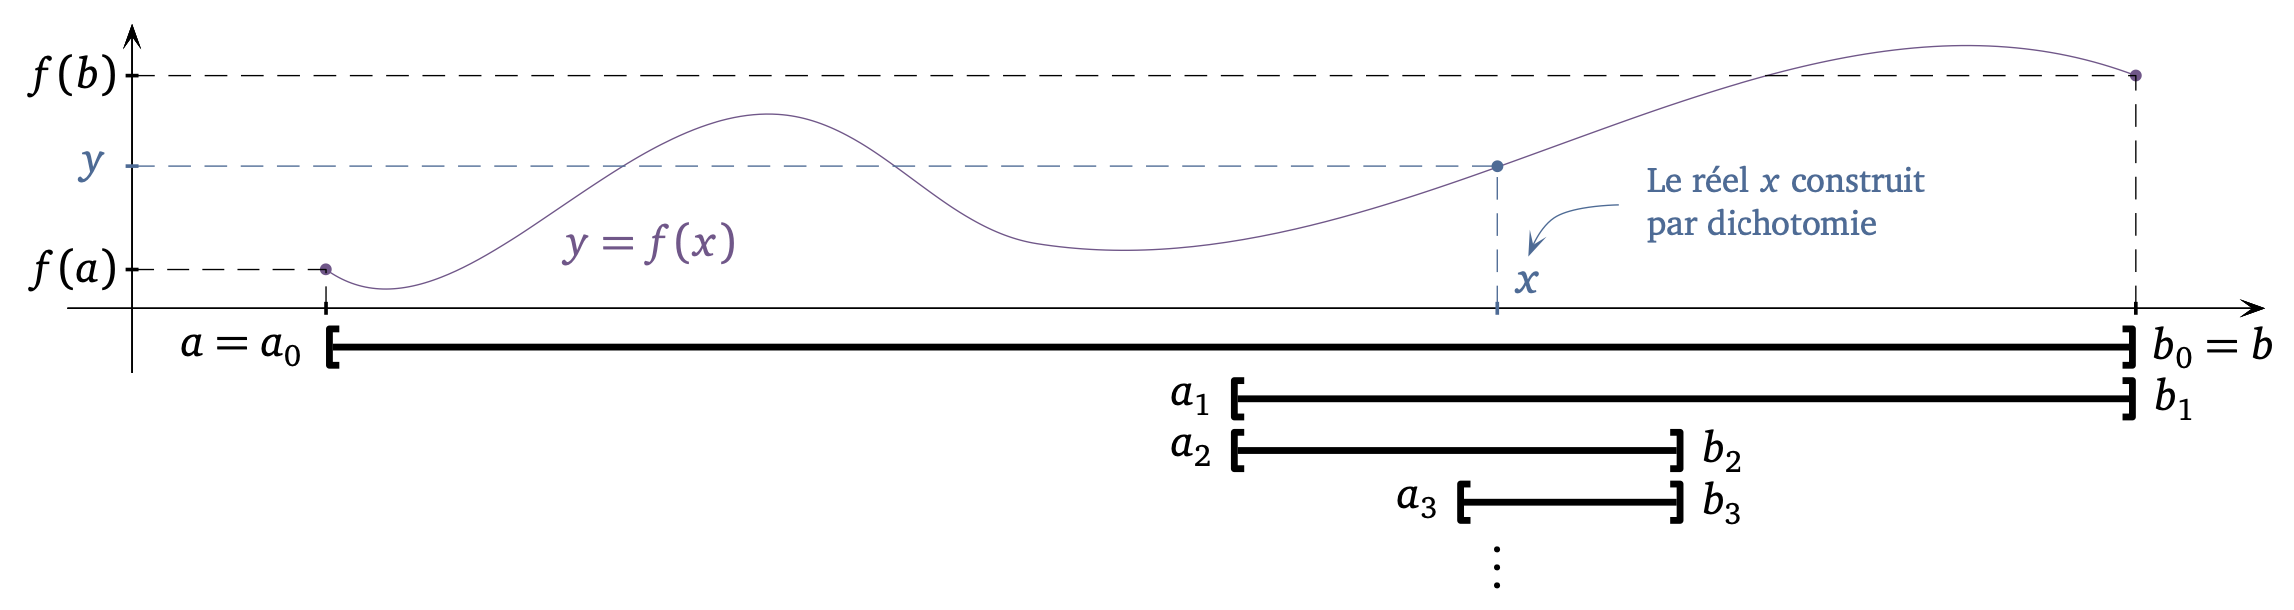
\includegraphics[width=0.9\textwidth]{../../commun/images/python-cours-dichotomie}
  \end{center}
On utilisera pour cela
l'algorithme de \emph{dichotomie} qui consiste à définir deux suites $(a_n)$ et $(b_n)$ en
commençant par poser $a_0\defeq a$, $b_0\defeq b$. Pour tout $n\in\N$, une fois $a_n$
et $b_n$ définis, on
définit $a_{n+1}$ et $b_{n+1}$ de la manière suivante~: on commence par calculer $f(c_n)$
où $c_n\defeq(a_n + b_n)/2$ et
\begin{itemize}
\item si $f(a_n)-y$ et $f(c_n)-y$ sont de signes distincts, on pose $a_{n+1}\defeq a_n$ et $b_{n+1}\defeq c_n$.
\item sinon, on pose $a_{n+1}\defeq c_n$ et $b_{n+1}\defeq b_n$.
\end{itemize}
Alors les suites $(a_n)$ et $(b_n)$ sont telles que pour tout $n\in\N$, il existe un
$x\in[a_n,b_n]$ tel que $f(x)=y$. De plus $b_n-a_n$ tend vers 0 lorsque $n$ tend vers $+\infty$.
\end{exoUnique}

\subsection{Assertion, test unitaire}

Afin de déceler au plus tôt la présence de bugs dans nos programmes, il est important
d'écrire des jeux de tests unitaires. Ces tests exécutent une fonction pure avec
des arguments dont la valeur de retour est connue; ils vérifient ainsi leur conformité. Par exemple,
pour vérifier que la fonction

\begin{pythoncodeline}
def factorielle(n):
    """factorielle(n: int) -> int"""
    fac = 1
    for k in range(1, n + 1):
        fac = fac * k
    return fac
\end{pythoncodeline}
\noindent nous renvoie bien la factorielle de $n$ pour tout $n\geq 0$,
on pourra vérifier que \verb!factorielle(0)! renvoie bien 1, \verb!factorielle(2)! renvoie bien 2 et
\verb!factorielle(5)! renvoie bien 120. Pour cela, on écrira

\begin{pythoncodeline}
assert factorielle(0) == 1
assert factorielle(2) == 2
assert factorielle(5) == 120
\end{pythoncodeline}
en dessous de la définition de notre fonction. De manière générale, le mot clé \verb!assert! est suivi d'une
expression qui doit s'évaluer en un booléen~: si ce booléen s'évalue en \verb!True!, l'instruction
\verb!assert! ne fait rien; sinon, elle lève une exception, ce qui se traduit par une erreur.

\subsection{Sortie anticipée}

Une fonction peut posséder plusieurs \verb_return_ dans son corps. Dans ce cas, le
premier \verb_return_ rencontré fait sortir de la fonction. Il est courant d'utiliser
cette propriété afin d'exprimer simplement certaines boucles. Par exemple, la fonction
suivante teste si une chaine de caractères possède un e.

\begin{pythoncodeline}
def possede_un_e(s):
    """possede_un_e(s: str) -> bool"""
    for k in range(len(s)):
        if s[k] == 'e':
            return True
    return False
\end{pythoncodeline}

\noindent
Dans cette fonction, la boucle a pour tâche de vérifier les caractères un à un. Si la
chaines de caractères $s$ possède un \og e \fg, il existe un indice $k\in\intere{0}{n-1}$
pour lequel \verb_s[k]_ est égal à \verb_'e'_; la fonction va exécuter la ligne 5,
renvoyer \verb_True_ et sortir immédiatement. Si la chaine de caractères
ne contient pas la lettre \og e \fg, la condition ligne 4 n'est jamais
satisfaite; on sort alors de la boucle et la dernière instruction renvoie \verb_False_.

\begin{pythoncode}
In [1]: s = "Puis, à la fin, nous saisirons pourquoi tout fut bati à partir d'un carcan si dur, d'un canon si tyrannisant. Tout naquit d'un souhait fou, d'un souhait nul : assouvir jusqu'au bout la fascination du cri vain, sortir du parcours rassurant du mot trop subit, trop confiant, trop commun, n'offrir au signifiant qu'un goulot, qu'un boyau, qu'un chas, si aminci, si fin, si aigu qu'on y voit aussitot sa justification."

In [2]: possede_un_e(s)
Out[2]: False
\end{pythoncode}

\noindent
Ce style de progammation, dans lequel il existe plusieurs points de sortie d'une fonction,
peut devenir plus difficile à comprendre. Il est donc découragé d'en abuser,
car c'est une source de bugs. Cependant, dans un exemple comme celui-ci, son usage est pleinement justifié.\\

Remarquons qu'une sortie anticipée casse le caractère inconditionnel d'une boucle \verb!for!, puisqu'on
ne sait plus avant de rentrer dans la boucle quel va être le nombre d'itérations. Cependant, elle
garde son caractère borné et est toujours assurée, soit de terminer totalement, soit
d'être interrompue par un \verb!return!.
\vspace{2ex}
\begin{exoUnique}
\exo
  \begin{questions}
  \question Écrire une fonction \verb!est_sous_mot_position(sm: str, s: str, k: int) -> bool! 
    prenant deux chaines de caractères \verb_sm_ et \verb_m_ et renvoyant \verb!True! si
    \verb!sm! est un sous-mot de \verb!s! commençant à la position $k$, et \verb!False! sinon.
    Par exemple \verb!est_sous_mot_position("th", "python", 2)! doit renvoyer \verb!True!.
    On supposera que le mot \verb!m! est assez grand pour contenir le sous-mot \verb!sm! à
    partir de la position $k$.
  \question En déduire une fonction \verb!est_sous_mot(sm: str, s: str) -> bool! renvoyant
    \verb!True! si \verb!sm! est un sous-mot de \verb!m! et \verb!False! sinon.
  \end{questions}
\end{exoUnique}
\vspace{2ex}
Notons que l'instruction \verb_break_ permet de sortir d'une boucle \verb!for/while!
(la plus intérieure s'il y en a plusieurs imbriquées), sans sortir de la fonction.
Son utilisation peut se justifier dans quelques rares cas,
par exemple si l'on souhaite écrire la fonction \verb!est_sous_mot(sm: str, s: str) -> bool! de
l'exercice précédent sans utiliser une fonction auxiliaire~:

\begin{pythoncodeline}
def est_sous_mot(sm, s):
    """est_sous_mot(sm: str, s: str) -> bool"""
    m = len(sm)
    n = len(s)
    for k in range(n - m + 1):
        found = True
        for i in range(m):
            if sm[i] != s[k + i]:
                found = False
                break
        if found:
            return True
    return False    
\end{pythoncodeline}

\begin{pythoncode}
In [3]: est_sous_mot("thon", "python")
Out[3]: True
\end{pythoncode}
\noindent
On l'utilisera cependant avec parcimonie, car il rend la compréhension d'un algorithme plus délicate. Il sera en
général beaucoup plus simple d'utiliser une fonction auxiliaire utilisant une sortie anticipée.





\section{Variable locale et globale}
\subsection{Variable locale}


Il est possible de créer des variables à l'intérieur d'une fonction. Ces variables sont
\emph{locales} à la fonction et sont détruites une fois sorti de cette dernière.

\begin{pythoncodeline}
def puissance_quatre(n):
    """puissance_quatre(n: int) -> int"""
    c = n * n
    return c * c
\end{pythoncodeline}

\begin{pythoncode}
In [1]: puissance_quatre(2)
Out[1]: 16

In [2]: c
(*@\textcolor{violet}{NameError: name 'c' is not defined}@*)
\end{pythoncode}

\noindent
Si la variable $c$ est définie avant l'appel de la fonction, sa valeur est
masquée lors de l'appel et on la retrouve une fois sorti de la fonction~:

\begin{pythoncode}
In [3]: c = 5

In [4]: puissance_quatre(2)
Out[4]: 16

In [5]: c
Out[5]: 5
\end{pythoncode}

\noindent
Pour comprendre ce phénomène, il est important de comprendre la notion de masquage des variables~:
une fois dans la fonction, ligne 4, juste avant d'exécuter l'instruction \verb_return_,
l'état du système est le suivant~:

\begin{pythoncode}
# sous-état local fonction  {c: 4, n: 2}
# sous-état global          {c: 5}
\end{pythoncode}

\noindent À ce moment précis, l'état du système est la superposition de deux sous-états~:
le sous-état du dessus a été créé lors de l'appel de notre fonction et celui du dessous
correspond au sous-état au moment de l'appel.
Cette superposition de sous-états est rendue possible par \emph{la pile d'appels}.
La variable à laquelle on accède est par défaut celle qui se situe dans le sous-état \emph{actif},
celui qui est le plus haut sur la pile. Par exemple, une fois à l'intérieur de notre fonction, la variable globale $c$ contenant
5 est masquée par la variable locale de même nom, contenant 4~: c'est cette dernière à laquelle
on accède. Une fois l'appel 
terminé, le sous-état local à l'appel est supprimé et on retrouve notre état initial.

\begin{pythoncode}
# sous-état global          {c: 5}
\end{pythoncode}

\noindent Ces sous-états sont agencés comme une pile d'assiettes~: lorsqu'on appelle une
fonction, une nouvelle \og assiette \fg est empilée au sommet de la pile; lorsque
cet appel se termine, cette assiette est supprimée.\\

Ce mécanisme permet à la fonction \verb+puissance_quatre+ de n'avoir aucun effet
sur l'état au niveau de l'appel.
Notons d'ailleurs que la variable $n$ est locale à la fonction~: elle est initialisée
avec l'argument effectif passé lors de son appel. Comme cette variable est locale,
on peut la modifier sans craindre d'effet de bord.

\begin{pythoncodeline}
def puissance_quatre(n):
    """puissance_quatre(n: int) -> int"""
    n = n * n
    return n * n
\end{pythoncodeline}

\begin{pythoncode}
In [6]: n = 2

In [7]: puissance_quatre(n)
Out[7]: 16

In [8]: n
Out[8]: 2
\end{pythoncode}

\subsection{Variable globale}

On appelle \emph{variable globale} toute variable définie dans le niveau le plus bas de la pile. Les \emph{variables locales} sont celles définies dans les niveaux supérieurs.
Si elles ne sont pas masquées, il est toujours possible d'accéder en lecture aux variables globales.

\begin{pythoncodeline}
b = 1

def f(a):
    """f(a: int) -> int"""
    return a + b
\end{pythoncodeline}

\begin{pythoncode}
In [1]: f(2)
Out[1]: 3  
\end{pythoncode}

\noindent Lorsque l'on est dans la fonction $f$
pour calculer \verb_f(2)_, ligne 5, juste avant le \verb_return_, l'état du système est donné par
\begin{pythoncode}
# sous-état local fonction  {a: 2}
# sous-état global                 {b: 1}
\end{pythoncode}
\noindent et l'accès à la variable globale $b$ est possible.\\

Cependant, par défaut, il n'est pas possible de changer la valeur d'une variable
qui n'est pas locale. Afin de pouvoir modifier une telle variable, il convient de la
déclarer à l'intérieur de la fonction comme \emph{globale} à l'aide du mot clé
\verb_global_.

\begin{pythoncodeline}
compteur = 0

def carre_mission_impossible(n):
    """carre_mission_impossible(n: int) -> int"""
    global compteur
    compteur = compteur + 1
    if compteur <= 2:
        return n * n
    else:
        return 0
\end{pythoncodeline}

\begin{pythoncode}
In [2]: carre_mission_impossible(2)
Out[2]: 4

In [3]: carre_mission_impossible(2)
Out[3]: 4

In [4]: carre_mission_impossible(2)
Out[4]: 0
\end{pythoncode}

\noindent Cette fonction, si vous l'utilisez, s'autodétruira après 2 appels.
Ce genre d'effet est très
difficilement compréhensible pour son utilisateur. On dit qu'elle est \emph{impure} car elle a un effet de bord. Comme elle ne renvoie pas
\verb!None!, ce comportement est surprenant.
C'est pourquoi, la modification de variables globales est un style de programmation à
proscrire.


\subsection{Composition de fonctions}

Une fonction peut elle-même appeler une autre fonction. On peut ainsi définir une fonction
calculant les coefficients binomiaux à l'aide d'une fonction calculant la factorielle
d'un entier.

\begin{pythoncodeline}
def factorielle(n):
    """factorielle(n: int) -> int"""
    fac = 1
    for k in range(1, n + 1):
        fac = fac * k
    return fac

def binome(k, n):
    """binome(k: int, n: int) -> int"""
    return factorielle(n) // (factorielle(k) * factorielle(n - k))
\end{pythoncodeline}

\noindent
Lors de l'exécution, la composition de fonctions fait apparaitre une succession de
sous-états sur plusieurs niveaux. Voyons cela sur un exemple simple~:

\begin{pythoncodeline}
def puissance_deux(n):
    """puissance_deux(n: int) -> int"""
    u = n * n
    return u

def puissance_quatre(n):
    """puissance_quatre(n: int) -> int"""
    u = puissance_deux(n)
    v = puissance_deux(u)
    return v
\end{pythoncodeline}


\begin{pythoncode}
In [1]: n = 2

In [2]: puissance_quatre(n)
Out[2]: 16
\end{pythoncode}

\noindent Lors du calcul de \verb+puissance_quatre(n)+, ligne 9, on appelle \verb!puissance_deux(u)! et
à l'intérieur de cette fonction, ligne 4, juste avant le \verb_return u_, le système est dans l'état suivant~:

\begin{pythoncode}
# sous-état local puissance_deux    {n: 4, u: 16}
# sous-état local puissance_quatre  {n: 2, u: 4}
# sous-état global                  {n: 2}
\end{pythoncode}
\noindent
La superposition de ces sous-états forme la pile d'appels.




% \subsection{Procédure, fonction pure}

% Les premiers langages de programmation, comme le \textsc{Fortran}, différenciaient fonctions
% et procédures. Les premières étaient pures et n'avaient aucun effet de bord. Les procédures
% avaient quant à elles pour but d'effectuer un
% effet de bord comme afficher une valeur à l'écran, imprimer un fichier, etc. Autrement dit,
% elles ne renvoyaient rien, mais changeaient \og l'état de la machine \fg. Les langages
% de programmation ont par la suite unifié ces deux notions, et le concept de procédure a été
% intégré au concept de fonction. Dans ce paradigme, les fonctions doivent obligatoirement renvoyer une
% valeur. On a donc inventé des type \og inutiles \fg qui n'ont qu'une seule valeur. En Python, ce type est appelé
% \verb_NoneType_ et il possède une unique valeur qui est \verb_None_. Pour
% programmer une procédure en Python, on écrit donc une fonction qui a un effet de
% bord et qui renvoie la valeur \verb_None_. En pratique, on n'écrira quasiment jamais de
% \verb_return None_ (qui peut s'écrire aussi \verb!return! sans argument)
% dans une fonction~: Python prend l'initiative de renvoyer
% \verb_None_ si une fonction se termine sans avoir rencontré de \verb_return_.\\

% Nous avons déjà rencontré une telle fonction. C'est la fonction \verb_print_.

% \begin{pythoncode}
% In [1]: print("hello, world")
% hello, world
% \end{pythoncode}

% \noindent
% Remarquons que contairement à ce qui se passe lorsqu'on écrit

% \begin{pythoncode}
% In [2]: "hello, world"
% Out[2]: 'hello, world'
% \end{pythoncode}

% \noindent
% dans le premier exemple, on a demandé d'afficher \verb_"hello, world"_ sur la sortie
% standard à l'aide d'un \verb_print_. Dans ce second exemple, Python a simplement
% renvoyé la valeur qu'on lui a donnée. Mais comme on travaille dans un \textsc{REPL},
% Python affiche cette valeur. Remarquons qu'en toute rigueur, Python devrait
% se comporter de la manière suivante en \textsc{REPL} lorsqu'on utilise la fonction
% \verb_print_. 

% \begin{pythoncode}
% In [3]: print("hello, world")
% hello, world
% Out[3]: None
% \end{pythoncode}

% \noindent
% Cependant, lorsqu'une fonction renvoie \verb_None_, la convention est de ne pas afficher
% cette valeur.\\

% Il est essentiel de ne pas confondre une fonction qui renvoie une valeur avec une
% fonction qui affiche cette valeur sur la sortie standard. Par exemple, les deux fonctions
% suivantes
% \begin{pythoncodeline}
% def foo(n):
%     """foo(n: int) -> int"""
%     return n + 1

% def bar(n):
%     """bar(n: int) -> NoneType"""
%     print(n + 1)
% \end{pythoncodeline}
% peuvent à première vue sembler similaires car dans un shell Python on a~:
% \begin{pythoncode}
% In [4]: foo(6)
% Out[4]: 7

% In [5]: bar(6)
% (*@\textcolor{violet}{7}@*)
% \end{pythoncode}
% Cependant, ces deux fonctions sont fondamentalement différentes. La première est composable
% alors que la seconde ne l'est pas.
% \begin{pythoncode}
% In [6]: 2 * foo(6)
% Out[6]: 14

% In [7]: 2 * bar(6)
% (*@\textcolor{violet}{7}@*)
% (*@\textcolor{violet}{TypeError: unsupported operand type(s) for +: 'NoneType' and 'int'}@*)
% \end{pythoncode}

% \noindent
% En prépa, il sera assez rare qu'on vous demande d'écrire des fonctions qui affichent
% une valeur à l'écran plutôt que de la renvoyer. Réfléchissez à deux fois si vous écrivez
% un \verb_print(ans)_ alors qu'on attend de vous plutôt un \verb_return ans_. Se tromper, c'est avoir l'assurance
% de perdre tous les points à la question.

% \begin{exoUnique}
% \exo Définir une fonction \verb!triangle(n: int) -> NoneType! qui prend en argument un
%   entier $n$ et qui dessine sur la sortie standard un triangle sur $n$ lignes.
% \begin{pythoncode}
% In [1]: triangle(5)
% (*@\textcolor{violet}{*}@*)
% (*@\textcolor{violet}{**}@*)
% (*@\textcolor{violet}{***}@*)
% (*@\textcolor{violet}{****}@*)
% (*@\textcolor{violet}{*****}@*)
% \end{pythoncode}
% \exo Écrire une fonction \verb_table(n: int) -> NoneType_ qui prend en entrée un entier
%   $n$ et qui affiche la table de $n$ de la manière suivante.
% \begin{pythoncode}
% In [2]: table(7)
% 0  *  7  =  0
% 1  *  7  =  7
% 2  *  7  =  14
% 3  *  7  =  21
% 4  *  7  =  28
% 5  *  7  =  35
% 6  *  7  =  42
% 7  *  7  =  49
% 8  *  7  =  56
% 9  *  7  =  63
% \end{pythoncode}
% \begin{sol}
% \begin{pythoncode}
% def table(n):
%     """table(n: int) -> NoneType"""
%     for k in range(10):
%         print(k, " * ", n, " = ", k * n)
% \end{pythoncode}
% \end{sol}
% \end{exoUnique}

% Pour le moment, nous n'avons vu que deux types de fonctions Python.
% \begin{itemize}
% \item Celles qui renvoient une valeur intéressante et qui n'ont aucun effet de bord. On
%   dit que de telles fonctions sont des fonctions \emph{pures}.
% \item Celles qui on en effet de bord, ne possèdent pas de \verb_return_ et renvoient
%   donc la valeur \verb_None_. On dit que de telles fonctions sont des \emph{procédures}.
% \end{itemize}
% Pour le moment, nous avons vu deux effets de bord~: afficher du texte sur la
% sortie standard et modifier une variable globale. Nous verrons bientôt un troisième effet
% de bord encore plus intéressant qui consiste à modifier une valeur mutable, comme une liste.\\

% Il est possible d'avoir des fonctions possédant des effets de bord qui renvoient une
% valeur différente de \verb_None_. De telles fonctions doivent être vues dans bien des cas de manière
% suspectes et il est important de les éviter. Cependant, nous verrons des cas où elles sont nécessaires mais
% attendez que l'énoncé vous demande explicitement d'écrire de telles fonctions avant de vous lancer dans
% leur écriture.

% \subsection{Renvoi de valeurs multiples, tuples}




% \begin{exercicepython}{}
% \begin{questions}
% \question On considère une suite $(u_n)$  définie par son premier terme $u_0=a$ et la relation de récurrence 
% \[\forall n \in \N \quad u_{n+1}=f(u_n)\] 
% \'Ecrire une fonction \verb_u(a, n, f)_ qui calcule et renvoie $u_n$.
% \question On considère une suite $(v_n)$  définie par ses premiers termes $u_0=a$, $u_1=b$, $u_2=c$ et la relation de récurrence
% \[\forall n \in\N \quad u_{n+3}=f(u_n,u_{n+1},u_{n+2})\] 
% \'Ecrire une fonction \verb_u(a, b, c, n, f)_ qui calcule et renvoie $u_n$. Combien cette fonction utilise-t-elle d'appels de $f$~? 
% \end{questions}
% \end{exercicepython}

% \begin{exercicepython}{}
% On suppose que $f$ est une fonction codée en Python par la fonction \verb_f_.
% \begin{questions} 
% \question \'Ecrire une fonction \verb_somme(f, n, m)_ qui calcule $\sum_{k=n}^m f(k)$.
% \question \'Ecrire une fonction \verb_produit(f, n, m)_ qui calcule $\prod_{k=n}^m f(k)$.
% \end{questions}
% \end{exercicepython}

% Voici enfin une liste d'exercices sur les fonctions~:

% \begin{exercicepython}{}
% Quel est l'effet des fonctions suivantes~? 

% \begin{pythoncode}
% def f(n):
%     for i in range(1, n + 1):
%         print(i * i)
% \end{pythoncode}



% \begin{pythoncode}
% def g(n):
%     res=0
%     for i range(1, n + 1): 
%         res = res + i 
%     return res
% \end{pythoncode}


% \begin{pythoncode}
% def h(n):
%     res=1
%     for i range(1, n + 1): 
%         res = res * i 
%     return res
% \end{pythoncode}

% \begin{pythoncode}
% def h(n, x):
%     res = 1
%     for i range(n - 1):
%         res = res * x
%     return res 
% \end{pythoncode}


% \begin{pythoncode}
% def s(n, valdeb):
%     res = valdeb
%     for i in range(1, n + 1) 
%         res = 3 * res**2 + 1
%     return res
% \end{pythoncode}

% \begin{pythoncode}
% def calculsuite(n, valdeb, f):
%     res = valdeb
%     for i in range(1, n + 1):
%         res = f(res)
%     return res
% def g(x):
%     return(3 * x * x + 1)
% calculsuite(4, 0, g)
% \end{pythoncode}
% \end{exercicepython}
\section{Programmation récursive}

Une fonction \emph{récursive} est une fonction qui s'appelle elle-même. Cette
possibilité donne naissance à un style d'algorithmes qu'on appelle programmation
récursive. L'idée essentielle derrière ce style est de \emph{réduire} la résolution
d'un problème à la résolution de problèmes similaires de tailles strictement inférieures.
Pour que ce principe fonctionne, il faut d'une part spécifier des problèmes de tailles
élémentaires, qu'on appelle \emph{cas de base}, et donner leurs solutions; il faut s'assurer
d'autre part que les réductions précédentes finissent toujours par rencontrer de
tels cas.

\subsection{Fonction récursive pure}

Commençons par un classique de la programmation récursive~: le calcul de $n!$.
\begin{itemize}
\item \emph{réduction}~: Si $n\geq 1$, alors $n! = n \times (n-1)!$.
\item \emph{cas de base}~: Sinon $n=0$ et $0!=1$.
\end{itemize}
La traduction en Python est immédiate.
\begin{pythoncodeline}
def factorielle(n):
    """factorielle(n: int) -> int"""
    if n >= 1:
        return n * factorielle(n - 1)
    else:
        return 1
\end{pythoncodeline}
\begin{pythoncode}
In [1]: factorielle(5)
Out[1]: 120
\end{pythoncode}

\vspace{2ex}
Sur le même principe, nous allons programmer la division euclidienne d'un entier
$a\in\N$ par $b\in\Ns$ en n'utilisant que des comparaisons, des additions et des
soustractions.
\begin{itemize}
\item \emph{réduction}~: Si $a\geq b$, on note $q$ et $r$
  le quotient et le reste de la division euclidienne de $a-b$ par $b$. Alors
  \[a-b=qb+r, \quad\text{donc}\quad a = (q+1)b+r.\]
  On en déduit que $q+1$ et $r$ sont le quotient et le reste de la division euclidienne de $a$
  par $b$.
\item \emph{cas de base}~: Sinon $0\leq a < b$ et le quotient de la division euclidienne
  de $a$ par $b$ est 0 et son reste est $a$.
\end{itemize}
On obtient ainsi la fonction~:
\begin{pythoncodeline}
def division(a, b):
    """division(a: int, b:int) -> tuple[int, int]"""
    if a >= b:
        q, r = division(a - b, b)
        return (q + 1, r)
    else:
        return (0, a)
\end{pythoncodeline}
\begin{pythoncode}
In [2]: division(23, 7)
Out[2]: (3, 2)
\end{pythoncode}

\begin{exoUnique}
\exo Définir de manière récursive la fonction \verb!puissance(x: int, n: int) -> int!
  calculant $x^n$ pour $n\in\N$. On utilisera le fait que $x^0=1$ et que si $n\geq 1$,
  alors $x^n= x^{n-1} x$.
\end{exoUnique}

\vspace{2ex}
Tout comme une boucle \verb!while! peut être infinie, une fonction récursive peut
ne jamais terminer. Prenons l'exemple de la fonction
\begin{pythoncodeline}
def est_pair(n):
    """est_pair(n: int) -> bool"""
    if n == 0:
        return True
    elif n == 1:
        return False
    else:
        return est_pair(n - 2)
\end{pythoncodeline}
\noindent
qui détermine si un entier $n$ est pair ou non. Elle fonctionne parfaitement pour
un entier $n\geq 0$, mais si on appelle \verb!est_pair(-1)!, la fonction
va appeler successivement \verb!est_pair! avec les valeurs $-3,-5,-7$, etc. Elle
ne terminera jamais et on obtiendra l'erreur
\begin{pythoncode}
In [3]: est_pair(-1)
(*@\textcolor{purple}{RecursionError: maximum recursion depth exceeded in comparison}@*)
\end{pythoncode}
Il faudra donc être attentif, lorsqu'on définit une fonction récursive, à ce que
tous les cas se réduisent à un cas de base en un nombre fini d'appels.\\


L'algorithme d'\emph{exponentiation rapide} permet de calculer efficacement $x^n$ pour $n\in\N$. Cet
algorithme se base sur les deux remarques suivantes~:
\begin{itemize}
\item \emph{réduction}~: Si $n>0$, pour calculer $x^n$, on effectue la division
  euclidienne de $n$ par 2. Il existe donc $p\in\N$ et $r\in\ens{0,1}$ tel que $n=2p+r$.
  On remarque ensuite que
\begin{itemize}
\item si $r=0$, c'est-à-dire si $n$ est pair, on a $x^n=(x^p)^2$.
\item si $r=1$, c'est-à-dire si $n$ est impair, on a $x^n=x(x^p)^2$. 
\end{itemize}
\item \emph{cas de base}~: On a $x^0=1$.
\end{itemize}
Ces deux remarques conduisent à l'algorithme suivant~:
\begin{pythoncodeline}
def expo_rapide(x, n):
    """expo_rapide(x: int, n: int) -> int"""
    if n == 0:
        return 1
    else:
        p = n // 2
        y = expo_rapide(x, p)
        if n % 2 == 0:
            return y * y
        else:
            return x * y * y
\end{pythoncodeline}

\noindent
L'algorithme d'exponentiation rapide permet de calculer $x^n$ de manière plus efficace
que l'algorithme naïf. Le calcul de $x^n$ se fait de manière naïve en $n-1$ multiplications.
Cependant, une récurrence immédiate montre qu'avec l'algorithme d'exponentiation rapide,
le calcul de $x^n$ pour $n\defeq 2^p$ nécessite seulement $2+p$ multiplications.
Ainsi, l'algorithme naïf a besoin de 1023 multiplications pour calculer $x^{1024}$ alors
que l'algorithme d'exponentiation rapide en a besoin seulement de 12, car $1024=2^{10}$.\\

Cet exemple nous permet de réaliser qu'une fonction récursive va le plus souvent
créer une pile d'appels conséquente. Par exemple, lors de l'appel
de \verb!expo_rapide(3, 4)!, on va finir par appeler récursivement
\verb!expo_rapide(3, 0)!. Lors de cet appel, une fois à la ligne 4, juste avant
le \verb!return 1!, la pile d'appels est dans l'état suivant~:

\begin{pythoncode}
# sous-état local expo_rapide(3, 0)  {x: 3, n: 0}
# sous-état local expo_rapide(3, 1)  {x: 3, n: 1, p: 0}
# sous-état local expo_rapide(3, 2)  {x: 3, n: 2, p: 1}
# sous-état local expo_rapide(3, 4)  {x: 3, n: 4, p: 2}
# sous-état global                   {}
\end{pythoncode}
\noindent Lors de l'appel précédent \verb!est_pair(-1)! qui ne terminait pas, l'erreur renvoyée était d'ailleurs
liée à cette pile d'appels qui était devenue trop grande. On parle de \emph{débordement
de la pile d'appels}, ou de \emph{stackoverflow} en anglais.


\subsection{Fonction récursive impérative}

Nous allons continuer en programmant le flocon de Von Koch. La génération 0
de ce flocon est un segment de longueur $a$,
\begin{center}
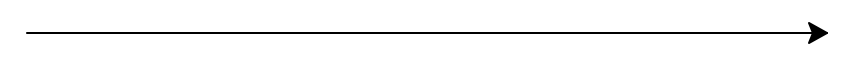
\includegraphics[width=0.4\textwidth]{../../commun/images/python-cours-koch-0}
\end{center}
la première génération est la figure suivante, le \og triangle \fg central étant
équilatéral,
\begin{center}
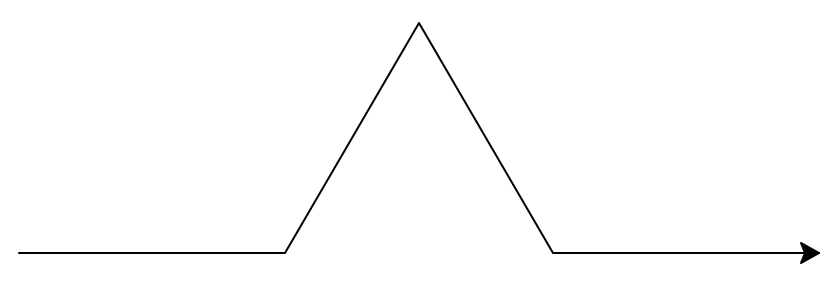
\includegraphics[width=0.4\textwidth]{../../commun/images/python-cours-koch-1}
\end{center}
puis la seconde génération est~:
\begin{center}
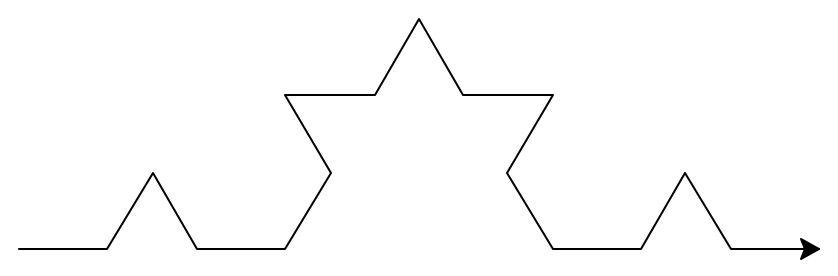
\includegraphics[width=0.4\textwidth]{../../commun/images/python-cours-koch-2}
\end{center}
Le but est d'écrire un programme dessinant la $n$-ième génération du flocon de
Von Koch de longueur $a$. On remarque évidemment le caractère récursif de sa
définition.
\begin{itemize}
\item \emph{réduction}~: Si $n\geq 1$, on dessine un flocon de Von Koch de longueur
  $a/3$ et de génération $n-1$, puis on tourne à gauche de 60 degrés, on
  dessine de nouveau le même flocon de Von Koch, on tourne à droite de 120 degrés,
  on dessine à nouveau un flocon de Von Koch, on tourne à gauche de 60 degrés
  et on dessine un dernier flocon.
\item \emph{cas de base}~: Si $n=0$, on trace un segment de longueur $a$.
\end{itemize}
On obtient ainsi le programme suivant~:
\begin{pythoncodeline}
import turtle as lg

def koch(a, n):
    if n == 0:
        lg.forward(a)
    else:
        koch(a / 3, n - 1)
        lg.left(60)
        koch(a / 3, n - 1)
        lg.right(120)
        koch(a / 3, n - 1)
        lg.left(60)
        koch(a / 3, n - 1)
\end{pythoncodeline}
Le tracé de la $4^e$ génération nous donne
\begin{center}
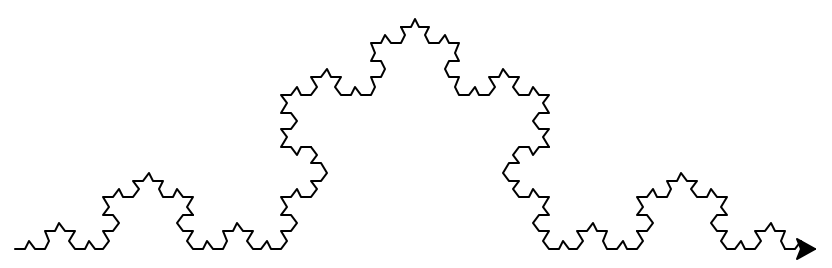
\includegraphics[width=0.4\textwidth]{../../commun/images/python-cours-koch-4}
\end{center}
Ce programme récursif est l'occasion de présenter l'arbre d'appels d'une fonction
récursive. Au sommet, nous avons la racine qui représente l'appel initial à notre
fonction. Cette fonction va elle-même s'appeler plusieurs fois et donc
générer des appels représentés dans l'arbre avec une profondeur de 1.
\begin{center}
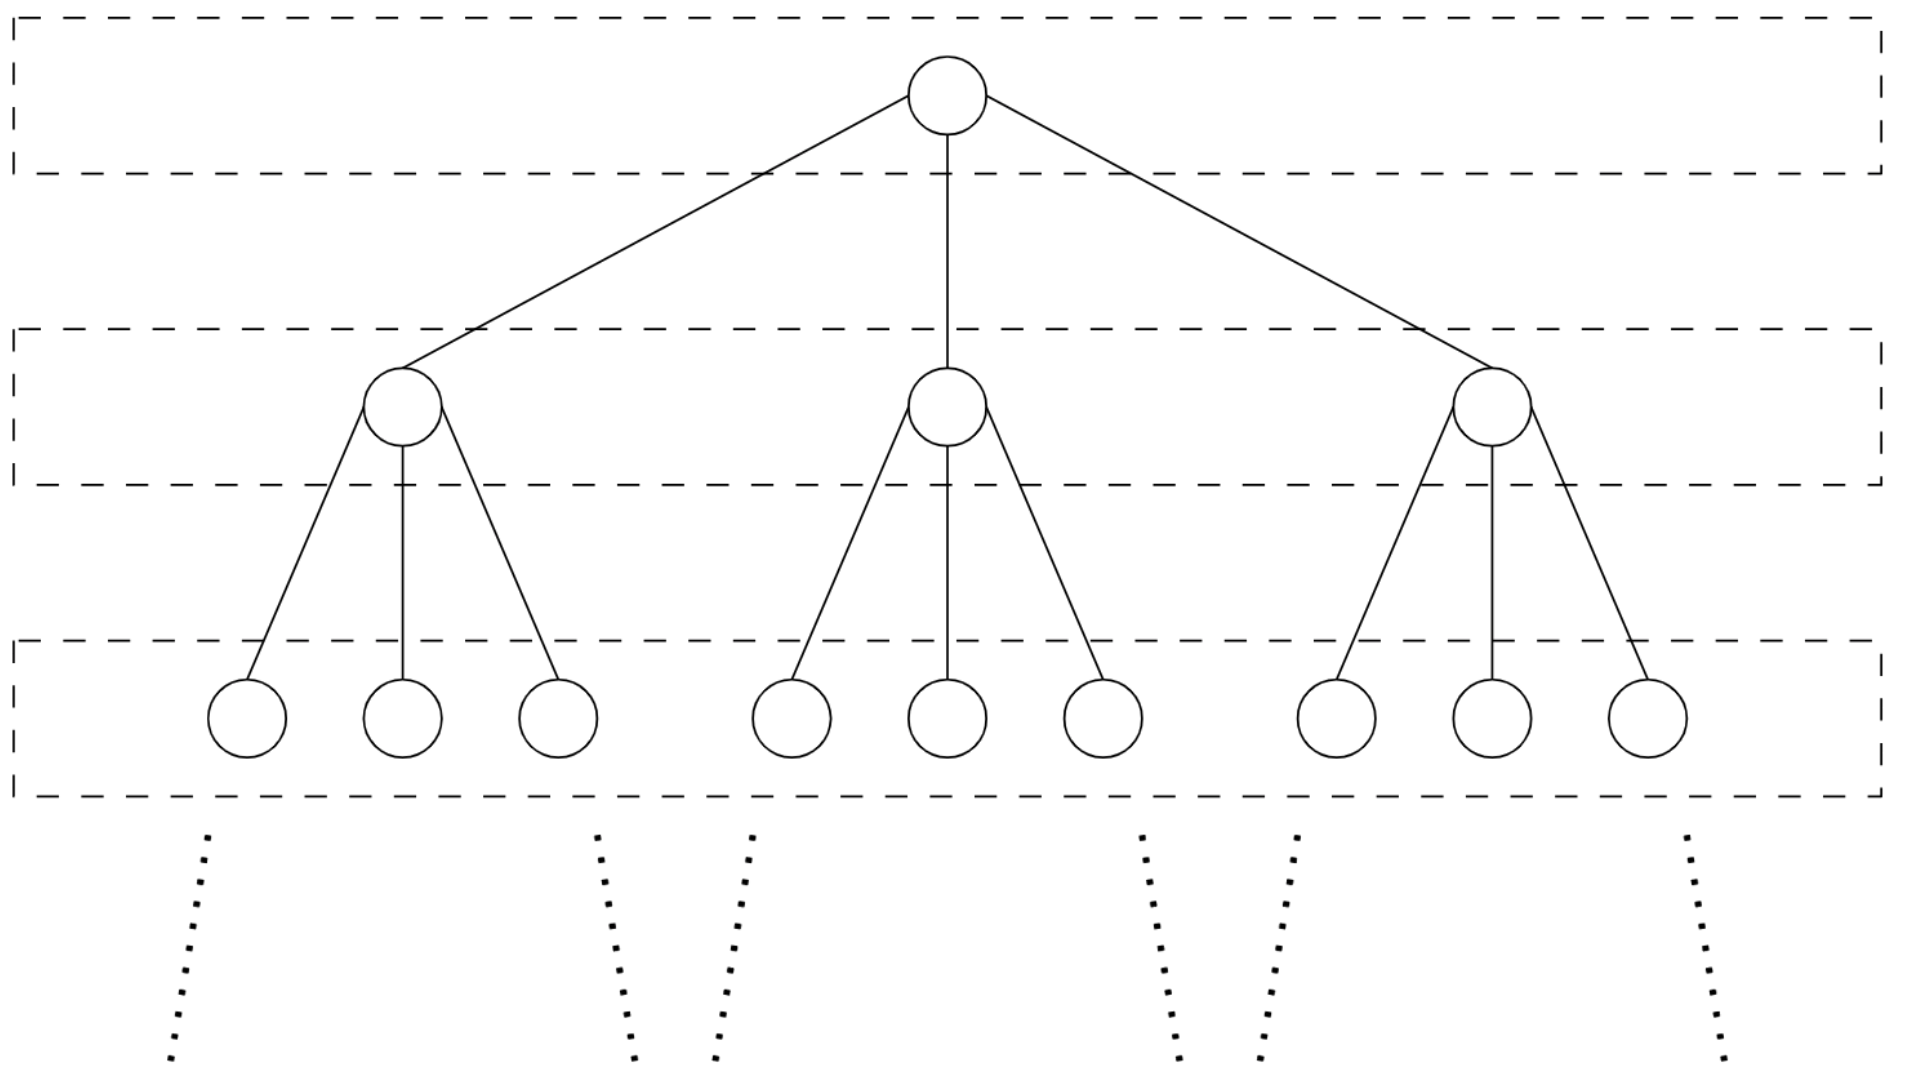
\includegraphics[width=0.6\textwidth]{../../commun/images/python-cours-arbre-appel}
\end{center}
Ces fonctions s'appellent elles-mêmes plusieurs fois, et ainsi de suite.\\

Nous allons maintenant nous atteler à la résolution d'un grand classique des jeux
mathématiques~: le jeu des tours de Hanoï, inventé par le mathématicien
Edouard Lucas. Ce jeu est constitué de trois tiges sur lesquelles sont enfilés $n$
disques de diamètres différents. Au début du jeu, ces disques sont tous positionnés
sur la première tige, du plus grand qui est en dessous, au plus petit. L'objectif
est de déplacer tous ces disques sur la troisième tige en respectant les règles
suivantes~:
\begin{itemize}
\item On ne peut déplacer qu'un disque à la fois.
\item On ne peut pas poser un disque sur un disque de diamètre inférieur.
\end{itemize}
\begin{center}
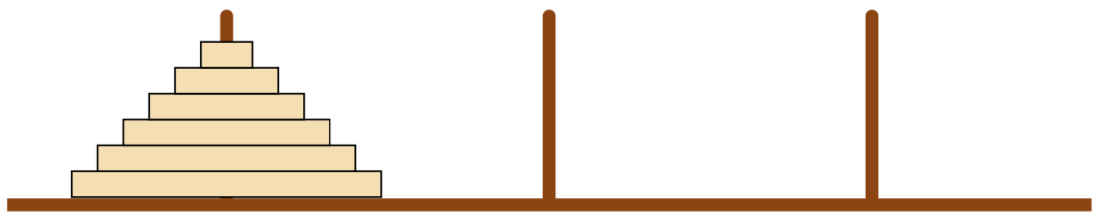
\includegraphics[width=0.6\textwidth]{../../Commun/Images/python-exos-rec-9.pdf}
\end{center}
Raisonnons par récurrence~: pour pouvoir déplacer le dernier disque, on déplace
les $n-1$ disques qui le couvrent sur la tige centrale. Une fois ces
déplacements effectués, nous pouvons déplacer le dernier disque sur la troisième
tige. Il reste alors à déplacer les $n-1$ autres disques vers la troisième tige.
\begin{center}
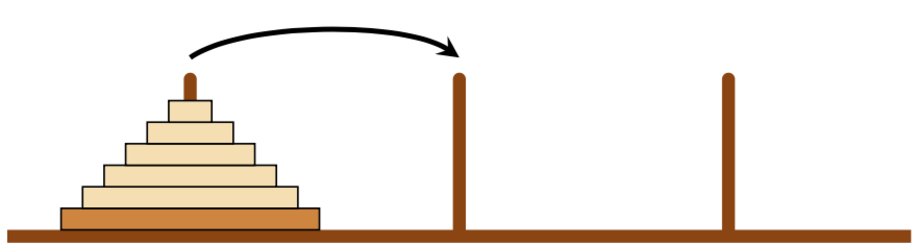
\includegraphics[width=0.6\textwidth]{../../Commun/Images/python-exos-rec-10.pdf}
\hspace{1cm}
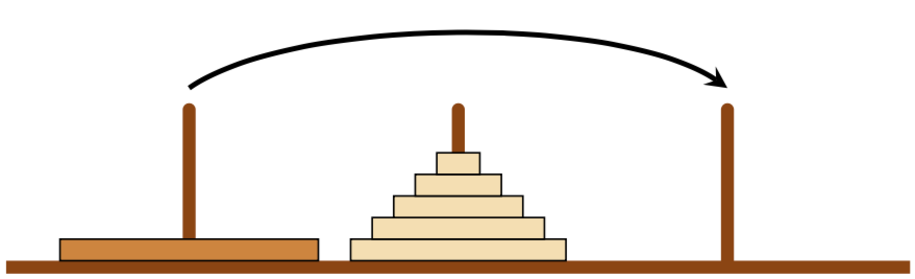
\includegraphics[width=0.6\textwidth]{../../Commun/Images/python-exos-rec-11.pdf}
\hspace{1cm}
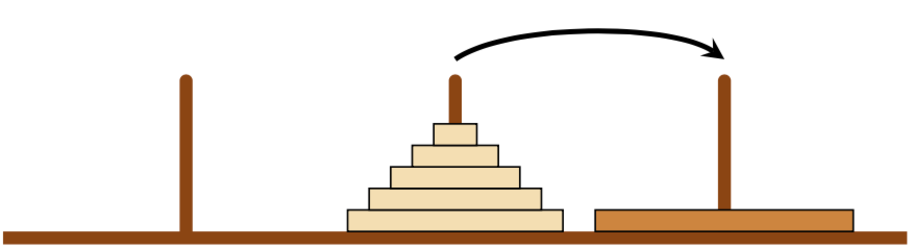
\includegraphics[width=0.6\textwidth]{../../Commun/Images/python-exos-rec-12.pdf}
\hspace{1cm}
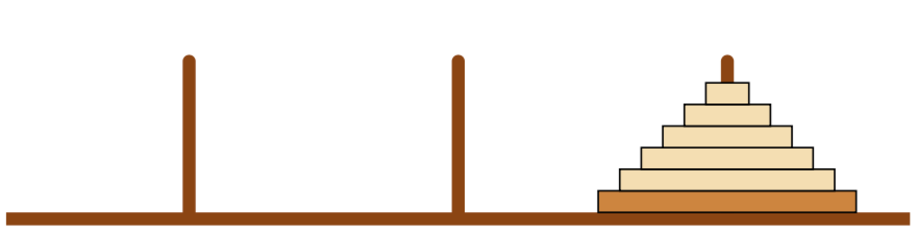
\includegraphics[width=0.6\textwidth]{../../Commun/Images/python-exos-rec-13.pdf}
\end{center}
Tout est dit~: pour pouvoir déplacer $n$ disques de la tige 1 vers la tige 3, il suffit de
savoir déplacer $n-1$ disques de la tige 1 vers la tige 2 puis de la tige 2 vers la tige 3.
Autrement dit, il suffit de généraliser le problème de manière à décrire le déplacement
de $n$ disques de la tige $i$ à la tige $k$ en utilisant la tige $j$ comme pivot. Ceci
conduit à la fonction suivante~:
\begin{pythoncodeline}
def hanoi(n, i, j, k):
    """hanoi(n: int, i: int, j: int, k: int) -> NoneType"""
    if n == 0:
        return None
    else:
        hanoi(n - 1, i, k, j)
        print("Déplacer le disque au sommet de la tige", i, "vers la tige", k)
        hanoi(n - 1, j, i, k)
\end{pythoncodeline}
\begin{pythoncode}
In [1]: hanoi(3, 1, 2, 3)
(*@\textcolor{purple}{Déplacer le disque au sommet de la tige 1 vers la tige 3}@*)
(*@\textcolor{purple}{Déplacer le disque au sommet de la tige 1 vers la tige 2}@*)
(*@\textcolor{purple}{Déplacer le disque au sommet de la tige 3 vers la tige 2}@*)
(*@\textcolor{purple}{Déplacer le disque au sommet de la tige 1 vers la tige 3}@*)
(*@\textcolor{purple}{Déplacer le disque au sommet de la tige 2 vers la tige 1}@*)
(*@\textcolor{purple}{Déplacer le disque au sommet de la tige 2 vers la tige 3}@*)
(*@\textcolor{purple}{Déplacer le disque au sommet de la tige 1 vers la tige 3}@*)
\end{pythoncode}


\begin{exoUnique}
\exo Déterminer le nombre de mouvements utilisés par l'algorithme précédent
  pour résoudre le problème des tours de Hanoï à $n$ disques.
\end{exoUnique}


\subsection{Fonctions mutuellement récursives}

Il est possible de définir des fonctions
\emph{mutuellement récursives} : l'exemple le plus simple serait
\[
  \begin{cases}
    f(0) \defeq 1 \\
    g(0) \defeq 0 \\
    \forall n \in \N\qsep f(n + 1) \defeq g(n) \\
    \forall n \in \N\qsep g(n + 1) \defeq f(n)
  \end{cases}
\]
Voici le code Python mettant en oeuvre ces fonctions~:
\begin{pythoncodeline}
def f(n):
    """f(n: int) -> int"""
    if n == 0:
        return 1
    else:
        return g(n - 1)

def g(n):
    """g(n: int) -> int"""
    if n == 0:
        return 0
    else:
        return f(n - 1)
\end{pythoncodeline}
% Pour programmer un tel couple de fonctions en \textsc{OCaml}, on utilise le mot-clé
% \verb!and! :
% \begin{camlcode}
% let rec f n =
%   if n = 0 then 1 else g (n - 1)
% and g n =
%   if n = 0 then 0 else f (n - 1)
% \end{camlcode}
% En remplaçant les $0$ et les $1$ par des booléens, on peut être plus concis :
% \begin{camlcode}
% let rec f n = (n = 0) || g (n - 1)
% and g n = (n <> 0) && f (n - 1)
% \end{camlcode}

\begin{exoUnique}
\exo
  De quelles fonctions élémentaires $f$ et $g$ sont-elles des
  implémentations tordues et inefficaces ?
\end{exoUnique}
\vspace{2ex}
Nous n'aurons pas très souvent besoin de définir des fonctions mutuellement
récursives, mais c'est quand même nécessaire de temps en temps.

%END_BOOK

\end{document}